%%%%%%%%%%%%%%%%%%%%%%%%%%%%%%%%%%%%%%%%%%%%%%%%%%%%%%%%%%%%%%%%%%%%%%%%%%%%%%%%
% intro.tex: Introduction to the thesis
%%%%%%%%%%%%%%%%%%%%%%%%%%%%%%%%%%%%%%%%%%%%%%%%%%%%%%%%%%%%%%%%%%%%%%%%%%%%%%%%
% Outline:
% - Active fluids
% - Emergent properties
% - Rheology: historical point of view
% - Collective motion: historical point of view
% - Directions: quantitative and geometry
%%%%%%%%%%%%%%%%%%%%%%%%%%%%%%%%%%%%%%%%%%%%%%%%%%%%%%%%%%%%%%%%%%%%%%%%%%%%%%%%




\chapter{Introduction}
\label{intro_chapter}
%%%%%%%%%%%%%%%%%%%%%%%%%%%%%%%%%%%%%%%%%%%%%%%%%%%%%%%%%%%%%%%%%%%%%%%%%%%%%%%%

\begin{itemize}

\item Chapter 1 briefly describe the history and significance of active fluid research.

\item Chapter 2 presents the experimental techniques used in this theis.

\item Chapter 3 talks about one of the emergent properties: reduced viscosity. Large portion of  this chapter have been published in \cite{Liu2019}.

\item Chapter 4 talks about another emergent property: giant number fluctuation. This work is under preparation for submission.

\item Chapter 5 presents the study on the transition from disordered state to active turbulence in light-powered bacterial suspensions. This work is conducted with a close collaboration with Yi Peng and Xiang Cheng. Large portions of this chapter has been published in \cite{Peng2020}. Yi Peng, Zhengyang Liu and Xiang Cheng conceived the experiment. Zhengyang Liu constructed the light-powered bacteria. Yi Peng performed the experiment. Zhengyang Liu and Yi Peng did the data analysis. All authors contribute to the model development and writing of the manuscript.

\item Chapter 6 summarizes the contributions of this thesis and provides the outlook on future research.

\item Appendix A shows details of the construction of light-powered \textit{E. coli}.

\item Appendix B provides details of several particle tracking tools I developed.

\item Appendix C shows details of photolithography.

\end{itemize}
%%%%%%%%%%%%%%%%%%%%%%%%%%%%%%%%%%%%%%%%%%%%%%%%%%%%%%%%%%%%%%%%%%%%%%%%%%%%%%%%


%%%%%%%%%%%%%%%%%%%%%%%%%%%%%%%%%%%%%%%%%%%%%%%%%%%%%%%%%%%%%%%%%%%%%%%%%%%%%%%%
\section{Active Matter and Active Fluids}
\label{active-fluids}

Active matter denotes a large group of active units which utilize ambient energy to achieve motions. Examples include flocking birds, schooling fish, herding beasts and even human crowds, down to actin filaments powered by motor proteins, bacteria and chemical reaction driven particles
\cite{Toner2005, Ramaswamy2010, Vicsek2012, Marchetti2013, Saintillan2013, Bechinger2016, Julicher2007}. The concept roots from a broader class of matter: soft matter, which includes polymers, surfactants and colloidal grains and shares common properties such as complexity and flexibility
\cite{DeGennes1992}. Like soft matter, active matter is also complex and flexible. What makes them more complex is the self-propulsion of each individual constituent, which endows them with more intrguing and counter-intuitive properties, challenging our understandings \cite{Glotzer2015}.

% such as abnormal rheology and emergent self-organized collective phenomena

Active fluids are suspensions of active agents such as cells, particles and biological macromolecules that are capable of utilizing chemical energy to sustain their self-propulsion. "fluids" in the name suggests the important role of the viscous hydrodynamic interaction and stress in the systems of interest. The first glimmering of active fluids dates back to 1969, when Finlayson and Scriven found that motion could spontaneously set in a previously still material without the intervention of outside forces, due to composition-dependent stress \cite{Finlayson1969}. However, the study on active fluids did not bloom, until 26 year later, when the seminal paper on modeling collective flocks came out \cite{Vicsek1995}. From then on, physicists are getting unprecedentedly intereted in biological phenomena, leading to the emergence of a new field of study - active fluids.

Early accomplishments in the research of active fluids include two successful theoretical predictions on the abnormal rheology and the spontaneous active turbulence \cite{Hatwalne2004, Simha2002}, which were then demonstrated in quite a few experiments
\cite{Dombrowski2004, Wensink2012, Rafai2010, Sokolov2009, Gachelin2013, Lopez2015}. From these beginnings, the field has been enjoying a vibrant interplay between experiment and theory, and more complex environment and geometrical constraints have been investigated \cite{Ramaswamy2019}. As of now, the study of active fluids has provided us with a good qualitative understanding of some biological processes, such as how active turbulence enhances nutrient transport.

There are two promising directions in active fluids. One is to get quantitative understanding of the novel properties.  These works will not only provide more accurate predictions on new systems, but also guide the engineering of artificial robots that can perform tasks in complex environment, such as drug delivery. Another direction is to invite chemistry and biology to collaborate on this highly interdisciplinary subject. A complete understanding of the behavior and properties of living systems will require the knowledge of biochemical signaling, which opens the door of an ambitious mission: elucidating tissue dynamics and developmental biology \cite{Marchetti2013, Curatolo2020}. The works that are to be described in Sec.~\ref{rheology-of-bacterial-suspensions-under-confinement},
\ref{giant-number-fluctuations-in-3-dimensional-space} and \ref{the-emergence-of-active-turbulence} are along the first direction: seeking more quantitative understanding of rheology and active turbulence of active fluids.

\begin{figure}[!htbp]
	\begin{center}
	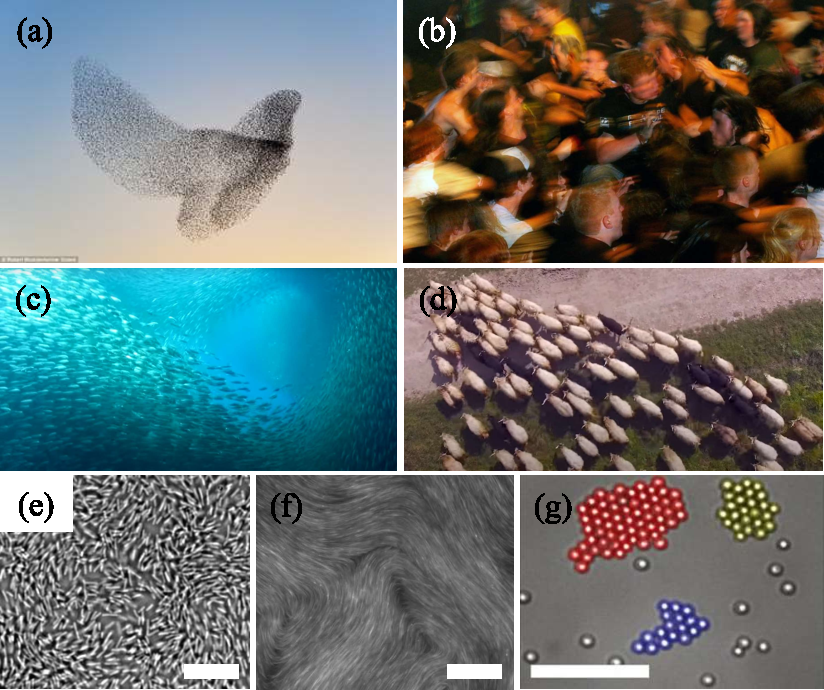
\includegraphics[width=5.5 in]{Figs/1-Intro/1.pdf}
	%select pdftexify command to run jpg or pdf files
	\end{center}
	\caption[Figure 1.1: Examples of living matters and active fluids.]
	{
  (a) Flocking birds, (b) people in a mosh pit at heavy metal converts, (c) schooling fish, (d) herding sheeps, (e) swarming bacteria (f) microtubule and (g) clustering active Janus particles.
  Scalebars in (e) and (g) are 10 \textmu m. Scalebar in (f) is 200 \textmu m. Images courtesy of Robert Wolstenhome (a), Ulrike Biets (b) \cite{Silverberg2013}, biographic (c, d), DeCamp (f) \cite{DeCamp2015} and Palacci (g) \cite{Palacci2013}.
	}
	\label{fig:1-1}
\end{figure}






\section{Novel Properties}
\label{emergent-properties}
Active fluids exhibit novel properties such as reduced viscosity and enhanced diffusion  \cite{Ramaswamy2010}. The reduced viscosity is explained by hydrodynamic stress and swim stress \cite{Saintillan2010}. And the enhanced diffusion is attributed to the interaction - steric collision or hydrodynamic perturbation - between tracer particles and active agents (swimmers)
\cite{Wu2000, Peng2016, Caspi2000, Morozov2014, Patteson2016, Leptos2009,
 Yang2016, Valeriani2011, Kurtuldu2011}.
In this section, the existing works regarding rheology and diffusion in active fluids are reviewed, and motivations for investigating the rheology of bacterial suspensions under confinement (Chap.~\ref{rheology-of-bacterial-suspensions-under-confinement}) will be discussed.


\subsection{Rheology}
\label{sec:rheology}


\subsectoin{Diffusion}
\label{sec:diffusion}
Polystyrene spherical tracer particles, typically a few microns across, show higher diffusivity in bacterial suspensions and active microtubules \cite{Wu2000, Caspi2000}.


\section{Collective motion}
The research on collective phenomena dates back to the 1980s, when flocking birds, schooling fish, herding beasts and even human crowds (Fig.~\ref{fig:1-1}a-d) were regarded as an orientationally ordered phase of living matter, in analogy with ferromagnetic spins
\cite{Reynolds1987, Vicsek1995, Narayan2007, Ward2008, Ballerini2008, Silverberg2013}. This idea has since evoked enormous research interest. More recently, besides macroscopic systems, smaller and more laboratory accessible model systems have joined. As examples, actin filaments powered by motor proteins and bacteria exhibit turbulence-like swirling patterns, and synthetic active colloids form dynamic clusters (Fig.~\ref{fig:1-1}e-g)
\cite{Dunkel2013, Wensink2012, Buttinoni2013, Palacci2013, Sanchez2012, Schaller2010, Sokolov2007}. Observations have revealed that most patterns of collective motion are universal in different systems. As of today, these universal patterns can be qualitatively reproduced by simple models with collision rules and noise. And quantitative description is developing with more observations available, which is bound to have impactful applications, including understanding the reaction of panic crowd and predicting the migration of fish schools
\cite{Vicsek2012}.
